\documentclass[11pt,a4paper]{article}

\usepackage[utf8]{inputenc}
\usepackage[T1]{fontenc}
\usepackage{amsmath,amssymb}
\usepackage{geometry}
\usepackage{hyperref}
\usepackage{caption}
\usepackage{subcaption}
\usepackage{tikz}
\usepackage{algorithm}
\usepackage{algpseudocode}
\usetikzlibrary{shapes, arrows.meta, positioning, calc, decorations.pathreplacing, backgrounds, patterns}

\geometry{margin=1in}

\title{\textbf{Sampling Method 1: Hard-First Two-Dimensional Tail Intersection}}
\author{Research Team}
\date{\today}

\begin{document}

\maketitle

\begin{abstract}
This document details Sampling Method 1 (referred to internally as \textit{Hard-First Sampling}), a targeted data selection strategy for Approximate Nearest Neighbor (ANN) index tuning. Rather than relying on pure uniform random sampling, which often underrepresents the difficult long-tail queries, Method 1 utilizes computationally cheap probes to map a large initial pool onto a two-dimensional performance plane. It explicitly derives thresholds from the Cumulative Distribution Functions (CDF) of coefficient of variation and convergence, harvesting the intersection of the worst-performing tails (bottom 5\%) before backfilling the remaining budget uniformly.
\end{abstract}

\section{Theoretical Formulation}

Let $\mathcal{D}$ represent the full dataset of vectors. To construct a representative yet challenging query sample $\mathcal{S}$ of size $N_{sample}$, we avoid the statistical dilution of hard queries by mining a much larger random pool $\mathcal{P} \subset \mathcal{D}$ of size $N_{pool}$ (where $N_{pool} \gg N_{sample}$).

\subsection{Cheap Algorithmic Probes}
For every query $q_i \in \mathcal{P}$, we execute a fast, low-budget adaptive search probe. Each probe yields a tuple of performance metrics:
\begin{enumerate}
    \item \textbf{Coefficient of Variation (CV)}: A dynamic internal confidence score indicating search difficulty.
    \item \textbf{Convergence}: The degree of search convergence achieved under the low-budget probe.
\end{enumerate}
Thus, every query is mapped to a 2D coordinate $(cv_i, conv_i)$.

\subsection{CDF-Based Tail Sorting and Intersection}
To identify the true worst-case queries without bias towards a single metric, we sort the pool independently along both axes. We formulate the empirical Cumulative Distribution Function (CDF) for both metrics. For a given value $x$, the CDF $F(x)$ represents the fraction of queries in the pool scoring less than or equal to $x$.

We define the bottom $5\%$ percentile thresholds by solving for the inverse CDF at $p = 0.05$:
\begin{align}
    cv^{(5\%)} &= F_{cv}^{-1}(0.05) \\
    conv^{(5\%)} &= F_{conv}^{-1}(0.05)
\end{align}

The hard query set $\mathcal{H}$ is strictly defined as the \textit{intersection} of both bottom-5\% tails:
\begin{equation}
    \mathcal{H} = \{ q_i \in \mathcal{P} \mid cv_i \leq cv^{(5\%)} \land conv_i \leq conv^{(5\%)} \}
\end{equation}

\subsection{Sample Construction}
The final sample $\mathcal{S}$ deterministically includes all identified hard queries. If the target budget $N_{sample}$ is not yet met, the remainder is populated by sampling uniformly without replacement from the ``easy'' pool:
\begin{equation}
    \mathcal{S} = \mathcal{H} \cup \text{UniformRandom}\Big(\mathcal{P} \setminus \mathcal{H}, \; \max(0, N_{sample} - |\mathcal{H}|)\Big)
\end{equation}

\section{Algorithmic Visualization}

The figures below illustrate the two-step geometric logic of Method 1. Figure~\ref{fig:cdf} explicitly shows the 1D threshold derivation, while Figure~\ref{fig:scatter} maps the 2D intersection dynamics.

% --- Figure 1: CDF ---
\begin{figure}[htbp]
    \centering
    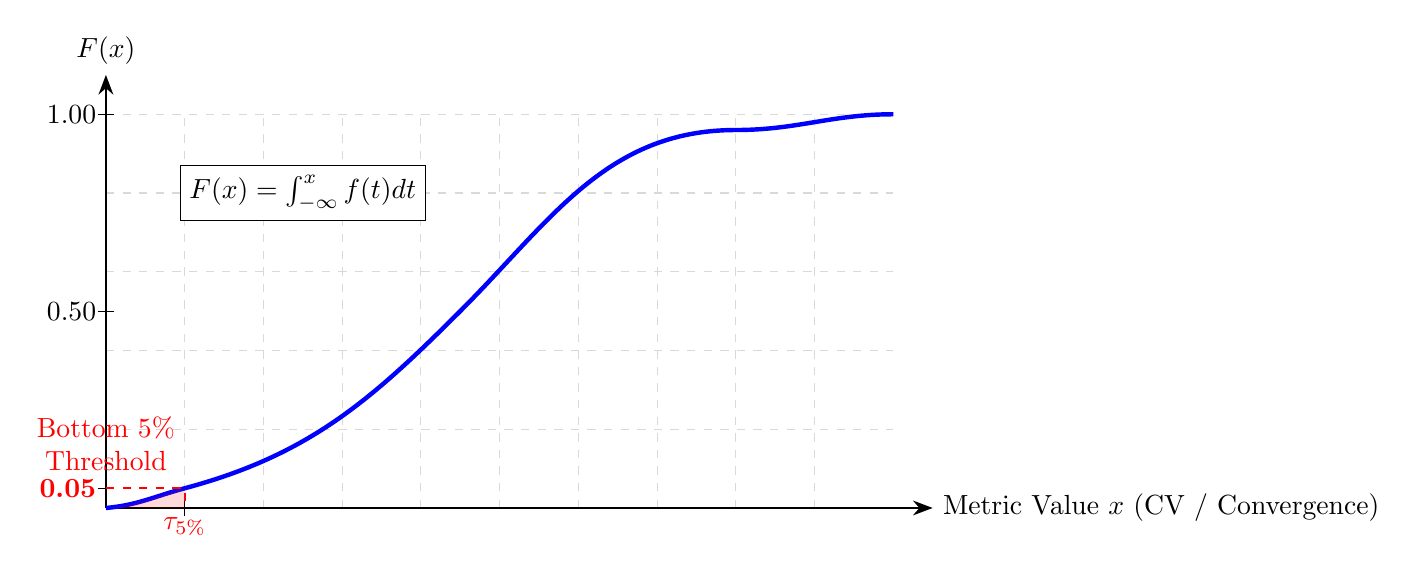
\begin{tikzpicture}[
        scale=1.0,
        axis/.style={thick, -{Stealth[length=2.5mm]}},
        gridline/.style={gray!30, thin, dashed},
    ]
        % Grid
        \foreach \y in {1, 2, 3, 4, 5} \draw[gridline] (0,\y) -- (10,\y);
        \foreach \x in {1, 2, ..., 9} \draw[gridline] (\x,0) -- (\x,5);
        
        % Axes
        \draw[axis] (0,0) -- (10.5,0) node[right] {Metric Value $x$ (CV / Convergence)};
        \draw[axis] (0,0) -- (0,5.5) node[above] {$F(x)$};
        
        % Ticks & Labels
        \draw (-0.1, 5) -- (0.1, 5) node[left=0.1cm] {1.00};
        \draw (-0.1, 2.5) -- (0.1, 2.5) node[left=0.1cm] {0.50};
        \draw (-0.1, 0.25) -- (0.1, 0.25) node[left=0.1cm, text=red, font=\bfseries] {0.05};
        
        \draw (1.0, -0.1) -- (1.0, 0.1) node[below=0.1cm, text=red, font=\bfseries] {$\tau_{5\%}$};
        
        % CDF Curve (Statistically realistic sigmoid shape)
        \draw[ultra thick, blue, smooth] (0,0) to[out=5, in=195] (1.0, 0.25) to[out=15, in=225] (4.5, 2.5) to[out=45, in=180] (8, 4.8) to[out=0, in=180] (10, 5);
        
        % 5% Intersection Lines
        \draw[dashed, red, thick] (0, 0.25) -- (1.0, 0.25) -- (1.0, 0);
        
        % Annotation
        \node[above left, text=red, align=center] at (1.0, 0.35) {Bottom 5\%\\Threshold};
        \node[draw, fill=white] at (2.5, 4.0) {$F(x) = \int_{-\infty}^{x} f(t) dt$};
        
        % Shade the 5% tail area under the curve
        \fill[red, opacity=0.15] (0,0) to[out=5, in=195] (1.0, 0.25) -- (1.0, 0) -- cycle;
    \end{tikzpicture}
    \caption{Derivation of the 5\% hardship threshold via the empirical Cumulative Distribution Function (CDF). The threshold $\tau_{5\%}$ explicitly isolates the hardest queries on a single axis.}
    \label{fig:cdf}
\end{figure}

% --- Figure 2: Pool Reduction (3-stage pipeline) ---
\begin{figure}[htbp]
    \centering
    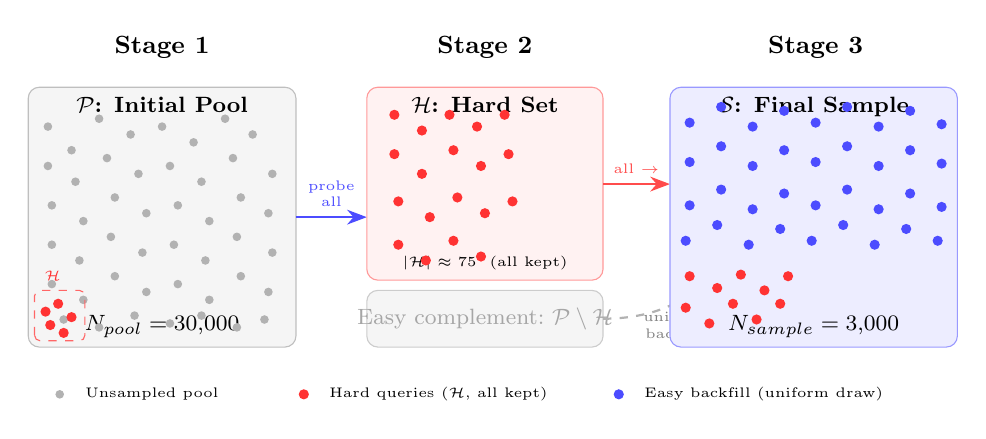
\begin{tikzpicture}[
        scale=1.0,
        arr/.style={-{Stealth[length=2.5mm]}, thick},
        smalldot/.style={circle, inner sep=1.1pt, fill=gray!60},
        reddot/.style={circle, inner sep=1.3pt, fill=red!80},
        bluedot/.style={circle, inner sep=1.3pt, fill=blue!70},
    ]

    %% ---- Stage 1: Initial Pool (30,000) ----
    \node[font=\bfseries\small] at (1.7, 3.8) {Stage 1};
    \draw[rounded corners=4pt, fill=gray!8, draw=gray!50]
        (0, 0) rectangle (3.4, 3.3);
    \node[anchor=north, font=\footnotesize\bfseries] at (1.7, 3.3)
        {$\mathcal{P}$: Initial Pool};
    \node[anchor=south, font=\footnotesize] at (1.7, 0)
        {$N_{pool} = 30{,}000$};

    % Dense gray dots = massive pool
    \foreach \px/\py in {
        0.25/2.8, 0.55/2.5, 0.9/2.9, 1.3/2.7, 1.7/2.8, 2.1/2.6, 2.5/2.9, 2.85/2.7,
        0.25/2.3, 0.6/2.1, 1.0/2.4, 1.4/2.2, 1.8/2.3, 2.2/2.1, 2.6/2.4, 3.1/2.2,
        0.3/1.8,  0.7/1.6, 1.1/1.9, 1.5/1.7, 1.9/1.8, 2.3/1.6, 2.7/1.9, 3.05/1.7,
        0.3/1.3,  0.65/1.1,1.05/1.4,1.45/1.2,1.85/1.3,2.25/1.1,2.65/1.4,3.1/1.2,
        0.3/0.8,  0.7/0.6, 1.1/0.9, 1.5/0.7, 1.9/0.8, 2.3/0.6, 2.7/0.9, 3.05/0.7,
        0.45/0.35,0.9/0.25,1.35/0.4,1.8/0.3, 2.2/0.4, 2.65/0.25,3.0/0.35
    } { \node[smalldot] at (\px, \py) {}; }

    % Red cluster in bottom-left corner = hard set buried inside pool
    \foreach \px/\py in {0.28/0.28, 0.45/0.18, 0.22/0.45, 0.55/0.38, 0.38/0.55} {
        \node[reddot] at (\px, \py) {};
    }
    \draw[red!60, dashed, rounded corners=2pt]
        (0.08, 0.08) rectangle (0.72, 0.72);
    \node[font=\tiny, red!80, anchor=south west] at (0.08, 0.72) {$\mathcal{H}$};

    %% ---- Arrow 1: Pool -> Stage 2 ----
    \draw[arr, blue!70] (3.4, 1.65) -- (4.3, 1.65)
        node[midway, above, font=\tiny, align=center]{probe\\all};

    %% ---- Stage 2: Hard Set + Easy Complement ----
    \node[font=\bfseries\small] at (5.8, 3.8) {Stage 2};

    % Hard Set box (top)
    \draw[rounded corners=4pt, fill=red!5, draw=red!40]
        (4.3, 0.85) rectangle (7.3, 3.3);
    \node[anchor=north, font=\footnotesize\bfseries] at (5.8, 3.3)
        {$\mathcal{H}$: Hard Set};
    \node[anchor=south, font=\tiny] at (5.8, 0.85)
        {$|\mathcal{H}| \approx 75$~~(all kept)};
    \foreach \px/\py in {
        4.65/2.95, 5.0/2.75, 5.35/2.95, 5.7/2.80, 6.05/2.95,
        4.65/2.45, 5.0/2.20, 5.4/2.50, 5.75/2.30, 6.1/2.45,
        4.7/1.85,  5.1/1.65, 5.45/1.90, 5.8/1.70, 6.15/1.85,
        4.7/1.30,  5.05/1.10,5.4/1.35, 5.75/1.15
    } { \node[reddot] at (\px, \py) {}; }

    % Easy Complement box (bottom)
    \draw[rounded corners=4pt, fill=gray!8, draw=gray!40]
        (4.3, 0.0) rectangle (7.3, 0.72);
    \node[font=\footnotesize, gray!70, align=center] at (5.8, 0.36)
        {Easy complement:~$\mathcal{P} \setminus \mathcal{H}$};

    %% ---- Arrow 2a: Hard set -> Final Sample (top) ----
    \draw[arr, red!70] (7.3, 2.07) -- (8.15, 2.07)
        node[midway, above, font=\tiny]{all $\rightarrow$};

    %% ---- Arrow 2b: Easy complement -> Final Sample (curved, bottom) ----
    \draw[arr, gray!60, dashed]
        (7.3, 0.36) .. controls (8.2, 0.36) and (8.6, 0.8) .. (8.6, 1.1)
        node[pos=0.45, below, font=\tiny, align=center, gray]{uniform\\backfill};

    %% ---- Stage 3: Final Sample (3,000) ----
    \node[font=\bfseries\small] at (10.0, 3.8) {Stage 3};
    \draw[rounded corners=4pt, fill=blue!7, draw=blue!40]
        (8.15, 0) rectangle (11.8, 3.3);
    \node[anchor=north, font=\footnotesize\bfseries] at (9.975, 3.3)
        {$\mathcal{S}$: Final Sample};
    \node[anchor=south, font=\footnotesize] at (9.975, 0)
        {$N_{sample} = 3{,}000$};

    % Red dots (hard queries) clustered near bottom of sample
    \foreach \px/\py in {
        8.35/0.50, 8.65/0.30, 8.95/0.55, 9.25/0.35, 9.55/0.55,
        8.40/0.90, 8.75/0.75, 9.05/0.92, 9.35/0.72, 9.65/0.90
    } { \node[reddot] at (\px, \py) {}; }

    % Blue dots (easy backfill) filling the rest
    \foreach \px/\py in {
        8.35/1.35, 8.75/1.55, 9.15/1.30, 9.55/1.50, 9.95/1.35,10.35/1.55,10.75/1.30,11.15/1.50,11.55/1.35,
        8.40/1.80, 8.80/2.00, 9.20/1.75, 9.60/1.95,10.00/1.80,10.40/2.00,10.80/1.75,11.20/1.95,11.60/1.78,
        8.40/2.35, 8.80/2.55, 9.20/2.30, 9.60/2.50,10.00/2.35,10.40/2.55,10.80/2.30,11.20/2.50,11.60/2.33,
        8.40/2.85, 8.80/3.05, 9.20/2.80, 9.60/3.00,10.00/2.85,10.40/3.05,10.80/2.80,11.20/3.00,11.60/2.83
    } { \node[bluedot] at (\px, \py) {}; }

    %% ---- Legend ----
    \node[smalldot] at (0.4, -0.6) {};
    \node[anchor=west, font=\tiny] at (0.6, -0.6) {Unsampled pool};
    \node[reddot] at (3.5, -0.6) {};
    \node[anchor=west, font=\tiny] at (3.7, -0.6) {Hard queries ($\mathcal{H}$, all kept)};
    \node[bluedot] at (7.5, -0.6) {};
    \node[anchor=west, font=\tiny] at (7.7, -0.6) {Easy backfill (uniform draw)};

    \end{tikzpicture}
    \caption{Three-stage Hard-First Sampling pipeline. \textbf{Stage~1}: A pool of $N_{pool}=30{,}000$ random vectors is probed cheaply to compute CV and Convergence for every candidate. \textbf{Stage~2}: The intersection of the bottom-5\% tails is extracted as the Hard Set $\mathcal{H}$ ($\approx$75 queries, all unconditionally retained); the remaining $\mathcal{P} \setminus \mathcal{H}$ forms the easy complement available for backfill. \textbf{Stage~3}: All hard queries are emitted first (red); the budget is then topped up by drawing uniformly from the easy complement (blue) until $N_{sample}=3{,}000$ is reached.}
    \label{fig:pool_reduction}
\end{figure}

% --- Figure 3: 2D Scatter Plot ---
\begin{figure}[htbp]
    \centering
    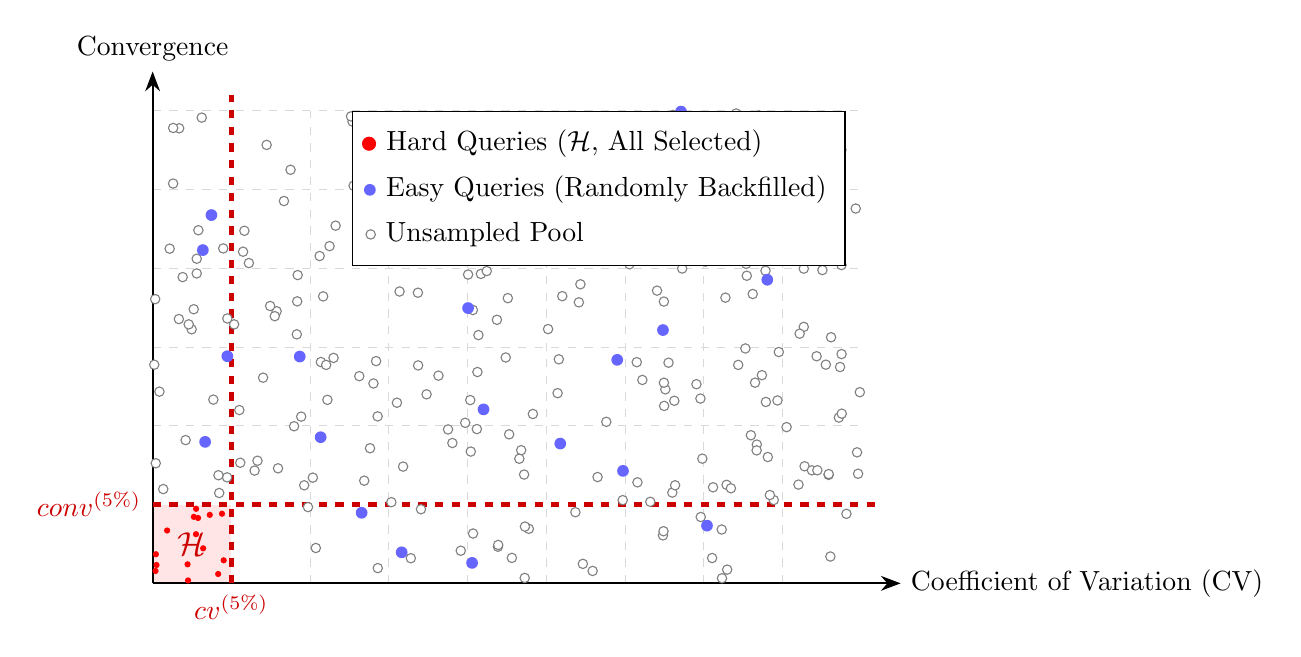
\begin{tikzpicture}[
        scale=1.0,
        axis/.style={thick, -{Stealth[length=2.5mm]}},
        gridline/.style={gray!30, thin, dashed},
        hard/.style={circle, fill=red, inner sep=1.8pt},
        easy/.style={circle, draw=gray, fill=white, inner sep=1.2pt},
        selected/.style={circle, fill=blue!60, inner sep=1.5pt}
    ]
    
    % Background Shade for Intersection
    \begin{scope}[on background layer]
        \fill[red!10] (0,0) rectangle (1.0, 1.0);
        \node[text=red!80!black, font=\large\bfseries] at (0.5, 0.5) {$\mathcal{H}$};
    \end{scope}

    % Grid
    \foreach \y in {1, 2, 3, 4, 5, 6} \draw[gridline] (0,\y) -- (9,\y);
    \foreach \x in {1, 2, 3, 4, 5, 6, 7, 8} \draw[gridline] (\x,0) -- (\x,6);

    % Axes
    \draw[axis] (0, 0) -- (9.5, 0) node[right] {Coefficient of Variation (CV)};
    \draw[axis] (0, 0) -- (0, 6.5) node[above] {Convergence};
    
    % Percentile Threshold Lines
    \draw[dashed, ultra thick, red!80!black] (1.0, 0) node[below] {$cv^{(5\%)}$} -- (1.0, 6.2);
    \draw[dashed, ultra thick, red!80!black] (0, 1.0) node[left] {$conv^{(5\%)}$} -- (9.2, 1.0);

    % Easy Pool (large background)
    \foreach \i in {1,...,200} {
        \pgfmathsetmacro{\x}{1.0 + rnd*8.0}
        \pgfmathsetmacro{\y}{1.0 + rnd*5.0}
        \node[easy] at (\x, \y) {};
    }
    
    % 1D Hard only (Bottom Right — high CV, low Convergence)
    \foreach \i in {1,...,25} {
        \pgfmathsetmacro{\x}{1.0 + rnd*8.0}
        \pgfmathsetmacro{\y}{rnd*0.95 + 0.02}
        \node[easy] at (\x, \y) {};
    }
    
    % 1D Hard only (Top Left — low CV, high Convergence)
    \foreach \i in {1,...,25} {
        \pgfmathsetmacro{\x}{rnd*0.95 + 0.02}
        \pgfmathsetmacro{\y}{1.0 + rnd*5.0}
        \node[easy] at (\x, \y) {};
    }
    
    % 2D Hard Intersection (bottom-left, all selected)
    \foreach \i in {1,...,15} {
        \pgfmathsetmacro{\x}{rnd*0.95 + 0.02}
        \pgfmathsetmacro{\y}{rnd*0.95 + 0.02}
        \node[hard, inner sep=0.8pt] at (\x, \y) {};
    }
    
    % Selected Easy (Blue backfill) across non-hard regions
    \foreach \i in {1,...,12} {
        \pgfmathsetmacro{\x}{1.0 + rnd*8.0}
        \pgfmathsetmacro{\y}{1.0 + rnd*5.0}
        \node[selected] at (\x, \y) {};
    }
    \foreach \i in {1,...,4} {
        \pgfmathsetmacro{\x}{1.0 + rnd*8.0}
        \pgfmathsetmacro{\y}{rnd*0.95 + 0.02}
        \node[selected] at (\x, \y) {};
    }
    \foreach \i in {1,...,4} {
        \pgfmathsetmacro{\x}{rnd*0.95 + 0.02}
        \pgfmathsetmacro{\y}{1.0 + rnd*5.0}
        \node[selected] at (\x, \y) {};
    }

    % Legend
    \matrix [draw, fill=white, anchor=north east] at (8.8, 6.0) {
      \node[hard, label={right:Hard Queries ($\mathcal{H}$, All Selected)}] {}; \\
      \node[selected, label={right:Easy Queries (Randomly Backfilled)}] {}; \\
      \node[easy, label={right:Unsampled Pool}] {}; \\
    };

    \end{tikzpicture}
    \caption{Two-dimensional metric intersection. The dashed lines represent the independent 5\% thresholds. Red points residing in the bottom-left quadrant ($\mathcal{H}$) strictly satisfy both hardship criteria and are prioritized. The blue points illustrate the uniform backfill sampling to reach the target budget $N_{sample}$.}
    \label{fig:scatter}
\end{figure}

\section{Methodological Advantages}
The implementation of Sampling Method 1 offers significant empirical advantages for index parameter tuning:
\begin{itemize}
    \item \textbf{Tail Stability:} By deliberately over-representing the bottom 5\% of topological difficulties, the optimization target heavily penalizes index structures that fail on edge cases, driving up tail-recall metrics (e.g., $\pi_{0.01}$).
    \item \textbf{Dimensional Independence:} Taking the \textit{intersection} of CV and Convergence (rather than relying on a blended heuristic) prevents false positives where a query has a low CV score simply due to local density variations but is geometrically trivial (yielding high Convergence).
\end{itemize}

\end{document}
